% !TEX encoding = UTF-8
% !TEX TS-program = pdflatex
% !TEX root = ../tesi.tex

\chapter{Lo stage}
\label{cap:stage}

%%%%%%%%%%%%%%%%%%%%%%%%%%%%%%%%%%%%%%%%%%%%%%%%%%%%%%%%%%%%%%%%%%%%%%%%%%%%%%%%%

\section{Il progetto}
Il progetto di stage, chiamato NFTLab, proposto dall'azienda Sync Lab consiste in un \emph{e-commerce} dedicato alla vendita di \textbf{NFT}. Prima di spiegare le varie funzionalità e caratteristiche di NFTLab, è doveroso fare una premessa e spiegare cosa sono gli NFT. \\

\begin{figure}[!h]
  \centering
  
\includegraphics[width=0.1\columnwidth]{capitolo2/nft-logo.png}
  \caption{Simbolo degli NFT}
\end{figure}

Nati nel 2017 in seguito alla richiesta di standardizzazione su blockchain Ethereum \emph{ERC721}, NFT è l'acronimo di \emph{Non Fungible Token} e per comprendere cosa sono e le loro possibili applicazioni, dobbiamo prima di tutto analizzare l'etimologia della parola. 
Un \emph{token} lessicale è un'insieme di caratteri che rappresentano qualsiasi cosa e il fatto che sia non fungibile implica che rappresenti un  di unico. 
In contrapposizione ai \emph{token} fungibili come le monete fisiche o le \gls{criptovalute}, i \emph{token} non fungibili non possono essere scambiati reciprocamente in quanto ognuno ha un valore che non è legato al \emph{token} in se, ma a quello che rappresenta.
Vengono salvati nella tecnologia \emph{blockchain} per semplificare la gestione dell'accesso e della proprietà, per assicurare l'unicità e l'impossibilità di contraffazione. \\

\noindent Gli NFT possono essere distinti dai token fungibili per le seguenti tre caratteristiche:
\begin{itemize}
  \item \textbf{Unico}: qualsiasi NFT viene definito da un codice univoco che lo rappresenta;
  \item \textbf{Raro}: questo è ciò che gli attribuisce il valore, in quanto se ce ne fossero di più varrebbero di meno;
  \item \textbf{Indivisibile}: gli NFT non possono essere suddivisi in parti, in quanto perderebbero il proprio valore. Possono essere detenuti, acquistati e venduti solo come entità intere.
\end{itemize}

\noindent Le applicazioni che possono avere sono di vario tipo, ma in generale ovunque ci sia bisogno di questi benefici:
\begin{itemize}
  \item \textbf{Fornire la proprietà}: consolidare il diritto di proprietà, visto che ogni NFT deve essere associato ad una persona;
  \item \textbf{Trasferibilità}: i diritti di proprietà di un NFT possono essere negoziati su vari mercati e scambiati facilmente;
  \item \textbf{Dimostrare l'autenticità}: utilizzando la tecnologia \emph{Blockchain} è possibile rassicurare i compratori dimostrando che il loro acquisto è autentico e originale.
\end{itemize}

L'ambito nel quale sono stati utilizzati sin da subito è l'arte digitale, dove c'è bisogno di dimostrare l'autenticità e la proprietà di una determinata opera per evitare contraffazioni.
Anche se esistono da tanti anni, sono diventati famosi solo verso la fine del 2020 e inizio 2021 grazie a siti che permettono il caricamento e la vendita di opere digitali sotto forma di NFT. Il sito più famoso ed utilizzato in questo ambito si chiama \emph{CryptoKitties}. Tutte le opere che si possono acquistare e vendere su \emph{CryptoKitties} riguardano dei gatti, a cui ogni autore può applicare delle particolarità che rendono la sua opera unica.

\begin{figure}[!tbph]
  
  \centering

  \begin{minipage}{0.5\textwidth}
    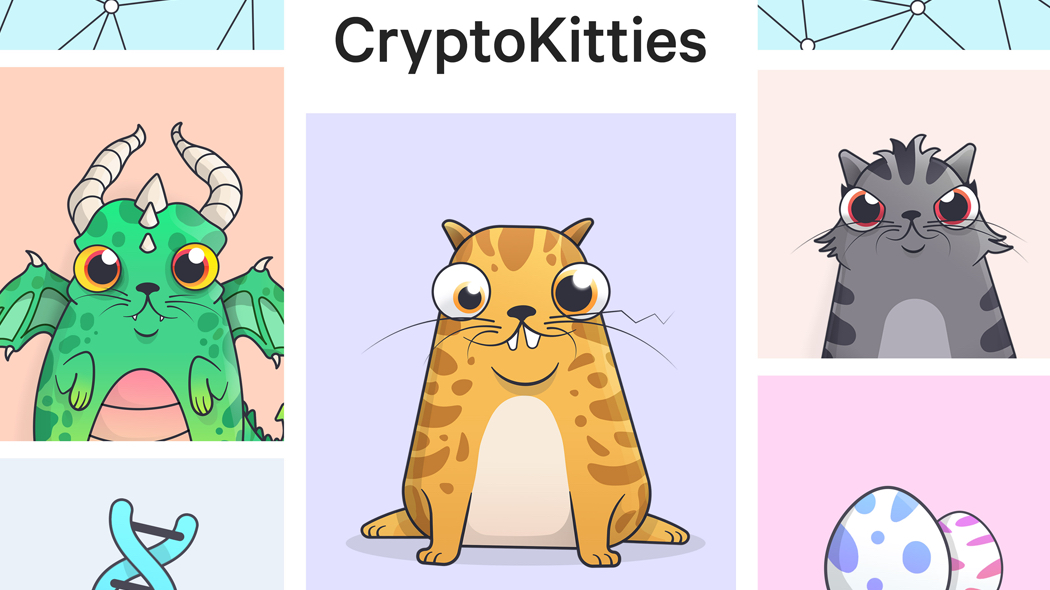
\includegraphics[width=\textwidth]{capitolo2/cryptokitties.jpg}
  \end{minipage}%
  \begin{minipage}{0.5\textwidth}
    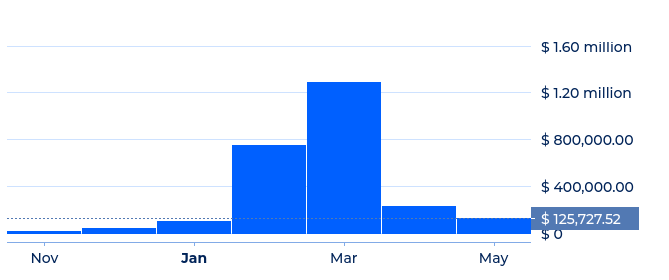
\includegraphics[width=\textwidth]{capitolo2/movimento-capitali-cryptokitties.png}
  \end{minipage}

  \begin{minipage}[t]{0.5\textwidth}
    \caption{Esempio di CryptoKitties}
    % \textbf{Fonte}: \href{https://www.cryptokitties.co}{https://www.cryptokitties.co}
  \end{minipage}%
  \begin{minipage}[t]{0.5\textwidth}
    \caption{Movimento di capitali sulla piattaforma CryptoKitties, anno 2020/2021}
    % \textbf{Fonte}: \href{https://coinranking.com/dapp/cryptokitties}{https://coinranking.com}
  \end{minipage}
\end{figure}

NFTLab è nato proprio da questo contesto. Oltre alle funzionalità di accesso e registrazione, permetterà agli utenti autenticati di caricare le proprie opere, che potranno essere qualsiasi tipo di file, aggiungendo un nome, una descrizione, le categorie facente parte, il prezzo e gli verrà anche assegnato un tipo in base al file. In seguito al caricamento verrà estratto il NFT e memorizzato in \emph{Blockchain}. 
Ogni utente potrà visualizzare le seguenti opere caricate da ogni utente, cercarle in base alle categorie di cui fanno parte, il loro tipo ed il nome, e comprarle, se autenticato. Quando visualizzerà i dettagli di un opera, in base al tipo del file, verrà mostrata un'anteprima di quest'ultima.
I dati di ogni opera possono essere cambiati dal proprietario, tranne l'opera in sè ed il tipo legato ad essa.

\begin{figure}[!h]
  \centering
  
\includegraphics[width=0.3\textwidth]{capitolo2/nftlab-logo.png}
  \caption{Logo di NFTLab}
\end{figure}

%%%%%%%%%%%%%%%%%%%%%%%%%%%%%%%%%%%%%%%%%%%%%%%%%%%%%%%%%%%%%%%%%%%%%%%%%%%%%%%%%

\section{Scelta dell'azienda}
La scelta di Sync Lab come azienda dove svolgere lo stage è avvenuta durante l'evento annuale, organizzato dall'Università degli Studi di Padova in associazione con gli imprenditori di AssIndustria VenetoCentro, chiamato \textbf{StageIT}. Questo evento, svoltosi online a causa della pandemia, permette alle aziende di presentare il loro ambito aziendale e anche i progetti proposti. Durante questo evento ho potuto incontrare varie aziende, analizzando di ognuna le opportunità che offriva. In seguito ho contattato e sono stato contattato varie aziende, le quali avevano il mio \textit{curriculum vitae} caricato in precedenza sulla piattaforma SIAGAS offerta dall'Università di Padova. Tra le varie aziende che mi hanno contattato c'è stata anche Sync Lab. \\

Il motivo principale che mi ha spinto a sceglierla come azienda dove svolgere lo stage è \textbf{il progetto}. Infatti, quasi tutti i progetti di stage che mi hanno proposto le altre aziende erano molto pratici, dove bisognava utilizzare un \textit{framework} per sviluppare siti web o applicazioni Android. Il progetto svolto con Sync Lab si discosta molto da quest'ottica, riuscendo ad unire perfettamente innovazione, aspetti teorici e aspetti pratici. Mi ha permesso di approfondire, sotto gli aspetti elencati in precedenza, la tecnologia \textit{blockchain} che ho sempre visto con molta curiosità, cercando di capire se fosse davvero solo una moda oppure poteva essere una tecnologia che avrebbe potuto rivoluzionare molti ambiti professionali. \\

Un altro motivo è stata \textbf{l'azienda Sync Lab}. Essendo un'azienda con un numero elevato di dipendenti e particolarmente strutturata, l'ho scelta con la speranza di poter vivere un ambiente lavorativo con grande esperienza e per potermi confrontare con persone molto più esperte di me sotto l'aspetto tecnico e tecnologico.

%%%%%%%%%%%%%%%%%%%%%%%%%%%%%%%%%%%%%%%%%%%%%%%%%%%%%%%%%%%%%%%%%%%%%%%%%%%%%%%%%

\section{Obiettivi dello stage}
Lo scopo del seguente stage è di sviluppare la parte di creazione e gestione degli NFT, utilizzando due \emph{blockchain}: Ethereum e Homoka. In seguito avrei dovuto scegliere la migliore e integrarla con il \emph{back-end} di NFTLab. L'obiettivo, perciò, consiste nello sviluppo di uno \emph{smart contract} per la gestione della compravendita di NFT e di una libreria Java che permetta a NFTLab di interagire con lo \emph{smart contract} caricato in \emph{blockchain}. \\

\noindent I prodotti attesi al termine dello stage sono i seguenti:
\begin{itemize}
  \item Una \textbf{relazione} dove verranno illustrate i seguenti punti:
  \begin{itemize}
    \item Le differenze nell'implementazione degli \emph{smart contract} per la gestione di NFT seguendo gli \emph{standard} delle due \emph{blockchain} sopra citate;
    \item Motivazioni che hanno spinto verso una soluzione piuttosto che verso l'altra;
    \item Spiegazione dell'architettura e le parti più complesse che sono state sviluppate.
  \end{itemize}
  \item Le \textbf{implementazioni degli \emph{smart contract}} richiesti, con la relativa libreria per l'interazione del \emph{back-end} con la \emph{blockchain}, dovranno essere consegnati in un'apposita \emph{repository} Git.
\end{itemize}

\section{Obiettivi personali}
In seguito ad una discussione avvenuta con il mio \emph{tutor} aziendale, l'ingegnere Fabio Pallaro, precedentemente all'inizio dello stage, sono stati definiti i seguenti obiettivi personali. Si farà riferimento ai requisiti secondo le seguenti notazioni:
\begin{itemize}
  \item \textbf{O}: per i requisiti obbligatori, vincolanti in quanto obiettivo primario richiesto dal committente;
  \item \textbf{D}: per i requisiti desiderabili, non vincolanti o strettamente necessari, ma dal riconoscibile valore aggiunto;
  \item \textbf{F}: per i requisiti facoltativi, rappresentanti valore aggiunto non strettamente competitivo.
\end{itemize}

\noindent La nomenclatura, perciò, sarà formata nel seguente modo:
\begin{center}
  (O|D|F)[0-9]+
\end{center}

\noindent Gli obiettivi di stage che ho conseguito sono riassunti di seguito:
\begin{longtable}{|c|l|}  
  \hline

  \textbf{Obiettivo} & \textbf{Descrizione} \\ \hline

  \textbf{Obbligatori} & \\

  O01       & Studio della tecnologia \emph{blockchain} \\
  O02       & Studio della \emph{blockchain} Ethereum \\
  O03       & Studio della \emph{blockchain} Hotmoka \\ 
  O04       & Studio del linguaggio Solidity \\ 
  O05       & Studio degli standard per la gestione degli (NFT) \\ 
  O06       & Implementazione del 80\% dei contratti per la gestione di NFT previsti \\
  
  \hline

  \textbf{Desiderabili} &  \\
  
  D01       & Implementazione del 100\% dei contratti previsti \\

  \hline

  \textbf{Facoltativi} & \\

  F01       & Implementazione dei \emph{test} relativi alle implementazioni realizzate \\

  \hline

  \caption{Obiettivi dello stage}

\end{longtable}

%%%%%%%%%%%%%%%%%%%%%%%%%%%%%%%%%%%%%%%%%%%%%%%%%%%%%%%%%%%%%%%%%%%%%%%%%%%%%%%%%

\section{Vincoli dello stage}
Prima di iniziare con lo stage, è stato redatto, insieme al mio \emph{tutor} aziendale Fabio Pallaro, il piano di lavoro dove sono stati specificati dei vincoli temporali e organizzativi. In seguito è stato approvato dal mio relatore, il professore Tullio Vardanega.

\subsection{Pianificazione temporale}
Lo stage si è svolto in una durata pari a 8 settimane, nel periodo che va dal 03-05-2021 al 25-06-2021, per un totale di 320 ore, ovvero 40 ore a settimana. Queste 8 settimane sono state divise in 3 periodi principali: il periodo di formazione, dove ho dovuto studiare i principi alla base delle varie \emph{blockchain} che sarei andato ad utilizzare, con i relativi linguaggi di programmazione per la stesura degli \emph{smart contract}; il periodo di sviluppo dove ho dovuto produrre i vari \emph{smart contract} e le relative integrazioni con il \emph{back-end}; il periodo di validazione, collaudo e presentazione del prodotto. \\

\noindent La pianificazione settimanale è la seguente: 
\begin{itemize}
  \item \textbf{Prima settimana (40 ore)}:
  \begin{itemize}
      \item Incontro con persone coinvolte nel progetto per discutere i requisiti e le richieste
      relativamente al sistema da sviluppare.
      \item Verifica credenziali e strumenti di lavoro assegnati.
      \item Studio dei concetti generali riguardanti la \emph{blockchain}.
  \end{itemize}
  \item \textbf{Seconda settimana (40 ore)}:
  \begin{itemize}
      \item Studio della \emph{blockchain} Ethereum.
  \end{itemize}
  \item \textbf{Terza settimana (40 ore)}:
  \begin{itemize}
      \item Studio del linguaggio Solidity per la definizione di \emph{smart contract}.
  \end{itemize}
  \item \textbf{Quarta settimana (40 ore)}:
  \begin{itemize}
      \item Studio e implementazione degli \emph{smart contract} per la gestione di NFT seguendo gli standard ERC su \emph{blockchain} Ethereum.
  \end{itemize}
  \item \textbf{Quinta settimana (40 ore)}:
  \begin{itemize}
      \item Studio della \emph{blockchain} Hotmoka.
  \end{itemize}
  \item \textbf{Sesta settimana (40 ore)}:
  \begin{itemize}
      \item Studio e implementazione degli \emph{smart contract} per la gestione di NFT seguendo gli standard Hotmoka.
  \end{itemize}
  \item \textbf{Settima settimana (40 ore)}:
  \begin{itemize}
      \item Conclusione codifica.
      \item Integrazione tra il \emph{back-end} e una delle due implementazioni sviluppate.
      \item Stesura della documentazione relativa al periodo di codifica.
  \end{itemize}
  \item \textbf{Ottava settimana - Conclusione (40 ore)}:
  \begin{itemize}
      \item Collaudo della soluzione e stesura della documentazione finale.
      \item Incontro di presentazione della soluzione con gli \emph{stakeholders}.
      \item \emph{Live demo} del lavoro di stage.
  \end{itemize}
\end{itemize}

\begin{figure}[!h]
  \centering
  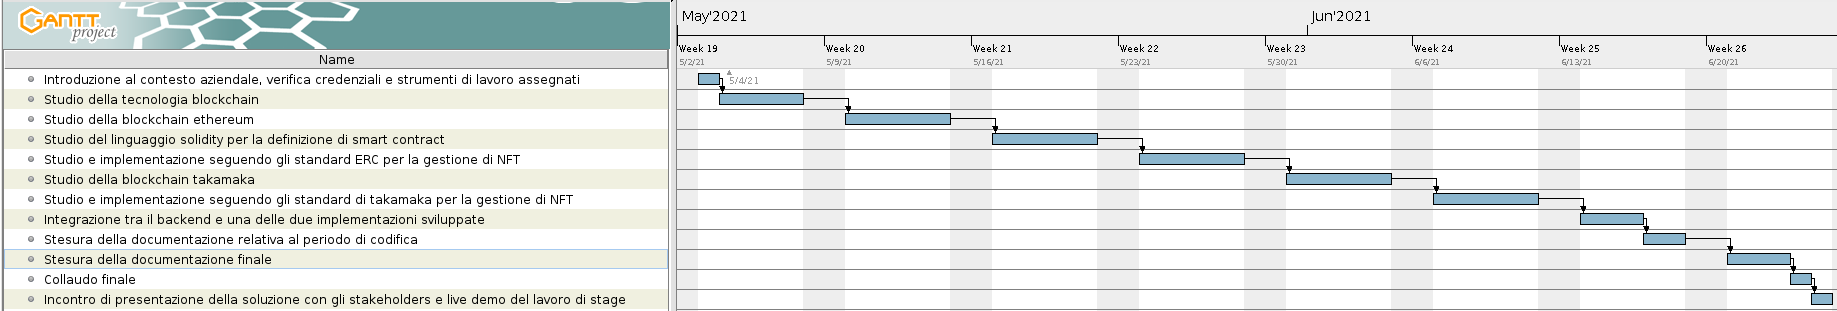
\includegraphics[width=\columnwidth]{capitolo2/gantt.png}
  \caption{Diagramma di Gantt relativo alla pianificazione dello stage}
\end{figure}

Per quanto riguarda la ripartizione oraria delle principali attività, qui si può vedere la tabella riassuntiva: \\

\begin{longtabu}{|c|X|}
	\hline

  \textbf{Durata in ore} & \textbf{Descrizione dell'attività} \\ \hline
  
	\textbf{160} & \textbf{Studio delle tecnologie} \\
  \textit{40} &
  Studio dei concetti generali riguardanti la \emph{blockchain} \\
  \textit{40} & 
  Studio della \emph{blockchain} Ethereum \\
  \textit{40} & 
  Studio del linguaggio Solidity per la definizione di \emph{smart contract} \\
  \textit{40} & 
  Studio della \emph{blockchain} Hotmoka \\
  
  \hline

  \textbf{80} & \textbf{Implementazione degli \emph{smart contract} per la gestione di NFT} \\ 
  \textit{40} & 
  Studio e implementazione degli \emph{smart contract} per la gestione di NFT seguendo gli standard ERC su \emph{blockchain} Ethereum \\
  \textit{40} & 
  Studio e implementazione degli \emph{smart contract} per la gestione di NFT seguendo gli standard Hotmoka \\
  
  \hline
  
  \textbf{24} & \textbf{Integrazione tra il backend e una delle due implementazioni sviluppate} \\
  \hline

  \textbf{40} & \textbf{Stesura documentazione} \\ 
  \textit{16} & 
  Stesura della documentazione relativa al periodo di codifica \\
  \textit{24} & 
  Stesura della documentazione finale \\

  \hline

  \textbf{16} & \textbf{Collaudo Finale}  \\ 
  \textit{13} & 
  Collaudo \\
  \textit{1} &
  Incontro di presentazione della piattaforma con gli \emph{stakeholders} \\
  \textit{2} & 
  Live demo del lavoro di stage \\
  \hline

  \textbf{Totale ore} & \multicolumn{1}{c}{\textbf{320}} \\ \hline

  \caption{Tabella riassuntiva delle ore per attività}
\end{longtabu}

\subsection{Vincoli organizzativi}
A causa della situazione pandemica ancora persistente, anche se in via di miglioramento, l'attività di stage è stata svolta in modalità mista. Sin dall'inizio dello stage è stato concordato con il mio \emph{tutor} aziendale, Fabio Pallaro, di fissare il lunedì come giorno obbligatorio di presenza in ufficio, in modo tale da poter eseguire lo \emph{sprint review}. 
Tutti gli altri giorni erano liberi e potevo scegliere personalmente se svolgere il lavoro in \emph{smart working}, oppure andare in ufficio. Per andare in ufficio dovevo prenotarmi minimo 2 giorni prima sulla piattaforma \emph{notion} e, nel caso ci fosse stato un numero considerevole di circa 10 persone gia prenotate, dovevo evitare di aggiungermi così da evitare il superamento delle 15 persone massime permesse dalla legge.
Personalmente, oltre al lunedì, andavo in ufficio anche il venerdì in modo tale da avere un contatto più diretto ed efficiente con gli altri membri del gruppo che hanno lavorato al progetto NFTLab.\\

Per mantenere attiva la comunicazione con il mio \textbf{\emph{tutor} aziendale}, è stato creato un registro delle attività condiviso dove, giornalmente, ho scritto i miei avanzamenti svolti nell'arco della giornata lavorativa. In seguito, ogni attività è stata verificata dal mio \emph{tutor} aziendale in modo tale da confermare la correttezza di quanto fatto. Per quanto riguarda il registro delle attività, ogni riga è stata organizzata nel seguente modo:
\begin{itemize}
  \item \textbf{Data}: data della giornata lavorativa interessata;
  \item \textbf{Descrizione}: breve descrizione dei progressi compiuti; 
  \item \textbf{Nota}: possibile nota del \emph{tutor} aziendale su quanto ho scritto nella descrizione;
  \item \textbf{Check del \emph{tutor} aziendale}: spunta che conferma la correttezza degli avanzamenti realizzati.
\end{itemize}

\begin{figure}[!h]
  \centering
  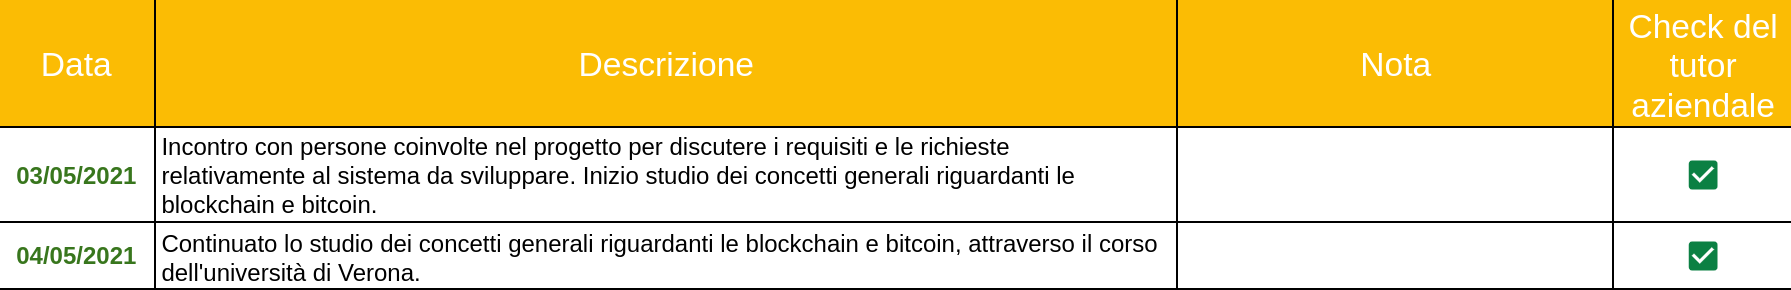
\includegraphics[width=\columnwidth]{capitolo2/registro-attivita.png}
  \caption{Estratto del registro delle attività}
\end{figure}

La comunicazione con il mio \textbf{\emph{tutor} interno}, ho provveduto ad informarlo tramite \emph{email} ogni 5 giorni lavorativi, riassumendo gli avanzamenti compiuti durante la settimana e specificando se fossero o meno coerenti con la pianificazione settimanale concordata nel piano di lavoro. Nel caso in cui ci fosse stata l'opportunità di cambiamento della pianificazione settimanale, avrei dovuto sottoporre la modifica alla sua approvazione, specificando le varie motivazioni. \\

La modalità di sviluppo adottata durante il mio stage, è stato fatto uso della metodologia \textbf{Scrum} in quanto è il metodo di sviluppo che viene adottato in tutti i progetti aziendali. Gli \emph{sprint} sono stati limitati ad una settimana e, come detto in precedenza, il lunedì era dedicato allo \emph{sprint review}. Questo mi ha permesso di analizzare e provare in prima persona la metodologia Scrum applicata in un ambito lavorativo e aziendale importante come lo è Sync Lab. \\

I \textbf{canali di comunicazione} utilizzati sono quelli che sono stati riportati in \$\{INSERIRE SEZIONE\}. Più nello specifico è stato utilizzato:
\begin{itemize}
  \item \textbf{Discord}: tramite questa piattaforma è stato possibile rimanere in comunicazione con il mio \emph{tutor} aziendale, per esporgli qualsiasi mio dubbio e riferirgli i problemi che ho incontrato che non sono riuscito a risolvere anche dopo un periodo considerevole di tempo, e con gli altri colleghi universitari che stavano lavorando sul progetto NFTLab;
  \item \textbf{Google Meet}: utilizzato per partecipare alle varie riunioni o incontri urgenti svolti con gli \emph{stakeholders};
  \item \textbf{Trello}: \emph{scrum board} utilizzata per l'organizzazione degli \emph{sprint} settimanali;
  
  \clearpage
  \begin{figure}[!h]
    \centering
    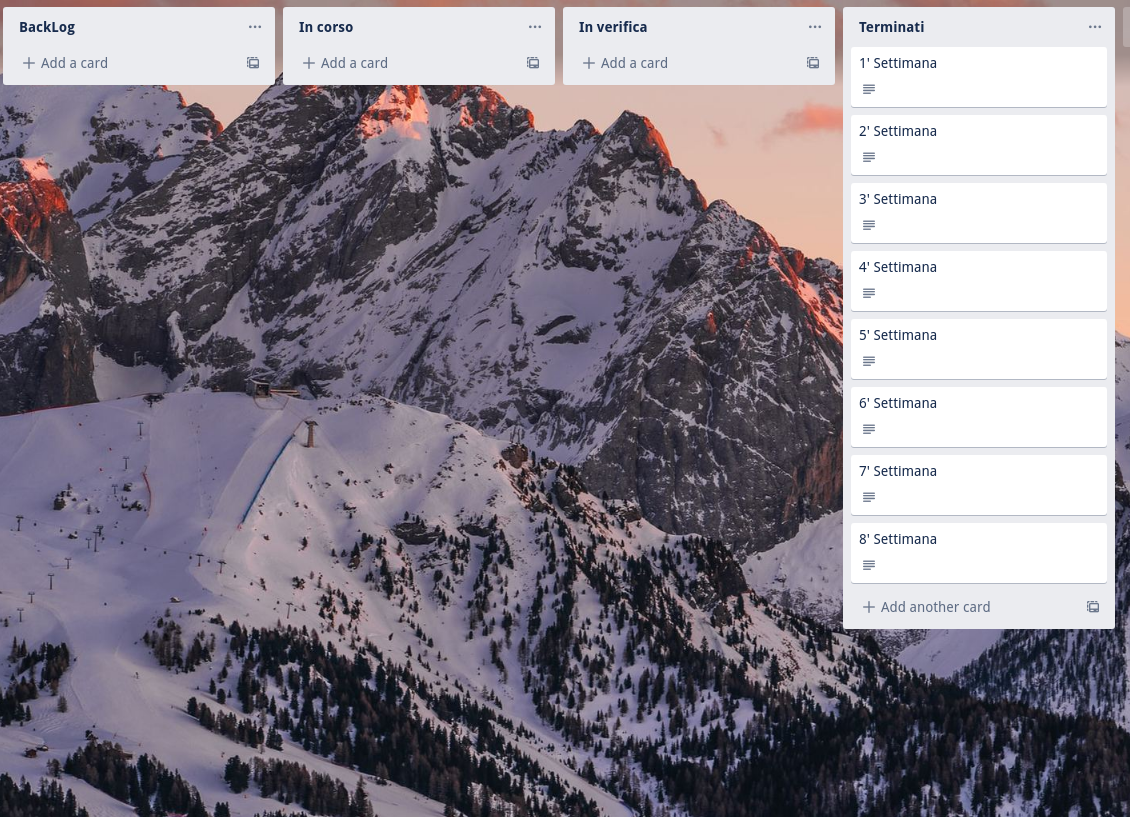
\includegraphics[width=0.8\textwidth]{capitolo2/trello-board.png}
    \caption{Gestione degli \emph{sprint} settimanali su Trello}
  \end{figure}

  \item \textbf{Notion}: impiegato, come già detto in precedenza, per la prenotazione della presenza in sede.
\end{itemize}

Per quanto riguarda la \textbf{gestione del codice}, non ci è stato imposto alcun vincolo da parte dell'azienda. Per questo motivo, è stata creata un'organizzazione sulla piattaforma \textbf{GitHub} dove sono raggruppate tutte le \emph{repository} e tutti gli artefatti prodotti. Il progetto è stato sviluppato con altre 4 persone che stavano facendo il percorso di stage dell'Università di Padova.

\begin{figure}[!h]
  \centering
  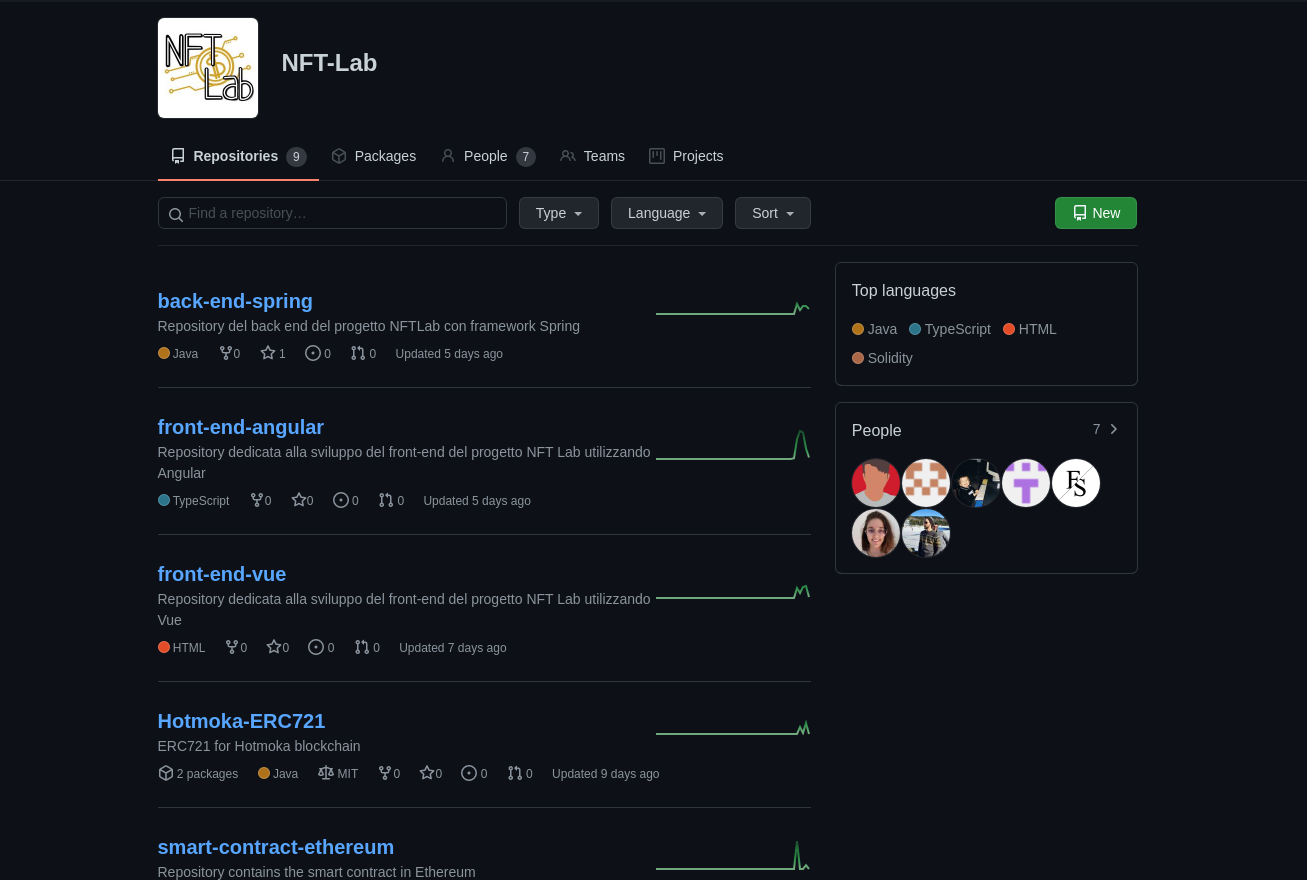
\includegraphics[width=0.8\textwidth]{capitolo2/github-organization.png}
  \caption{Organizzazione NFTLab su GitHub}
\end{figure}
